\documentclass[tikz,border=5pt]{standalone}
\usepackage{hsbcommon}
\makeatletter\AtBeginDocument{\@buildstepset{1,2,3}}\makeatother
\usetikzlibrary{calc}
\usepackage{etoolbox}

\begin{document}

\makeatletter
\@ifundefined{c@innerCnt}{\newcounter{innerCnt}}{}
\makeatother
\providecommand{\innerlist}{}

\providecommand{\innerbox}[1]{\listadd{\innerlist}{#1}}
\providecommand{\countone}[1]{\stepcounter{innerCnt}}

\providecommand{\drawinneritem}[1]{%
  \stepcounter{innerCnt}%
  \pgfmathsetmacro{\ytop}{\OY+\OH-(\value{innerCnt}-1)*\CH}%
  \pgfmathsetmacro{\ybot}{\OY+\OH-\value{innerCnt}*\CH}%
  \node at ({\OX+\OW/2},{(\ytop+\ybot)/2}) {
  \parbox{2.5cm}{\centering #1}
  };
  \ifnum\value{innerCnt}<\N
    \draw (\OX,\ybot) -- (\OX+\OW,\ybot);
  \fi
}

% #1 #2 = x,y of outer box   #3 = width   #4 = height   #5 = content
\providecommand{\outerbox}[5]{%
  \renewcommand{\innerlist}{}%
  #5\relax
  \setcounter{innerCnt}{0}%
  \forlistloop{\countone}{\innerlist}%
  \edef\N{\arabic{innerCnt}}%
  \pgfmathsetmacro{\OX}{#1}\pgfmathsetmacro{\OY}{#2}%
  \pgfmathsetmacro{\OW}{#3}\pgfmathsetmacro{\OH}{#4}%
  \pgfmathsetmacro{\CH}{\OH/\N}%
  \draw (\OX,\OY) rectangle ++(\OW,\OH);
  \setcounter{innerCnt}{0}%
  \forlistloop{\drawinneritem}{\innerlist}%
}

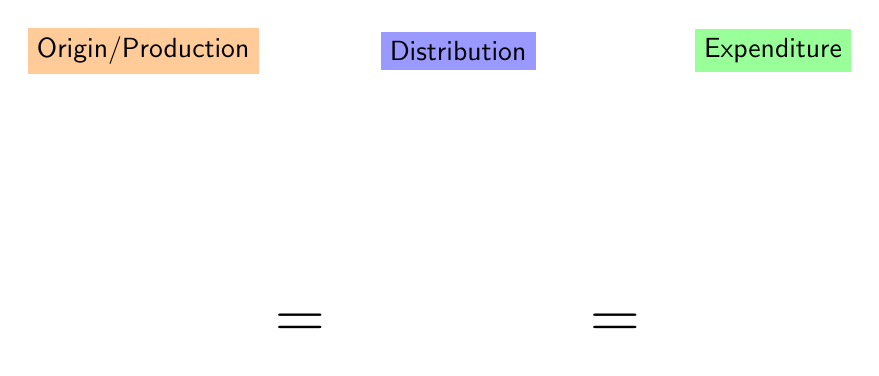
\begin{tikzpicture}
    \tikzset{every node/.style={font=\sffamily},>=latex}

\ifstep{1}{
    
    \node[fill=orange!40] at (1.5,6.5) {Origin/Production};
    \outerbox{0}{0}{3}{6}{
        \innerbox{Gross Value Added (GVA) in products, various sectors}
        \innerbox{GVA in services, various sectors}
        \innerbox{net taxes on products and services
        }
        }
}

\ifstep{1}{
    \ifstep{2}{
    \node at (3.5,3) {\Huge $=$};
    }
}
    
\ifstep{2}{
    \node[fill=blue!40] at (5.5,6.5) {Distribution};
    \outerbox{4}{0}{3}{6}{
        \innerbox{wages, salaries}
        \innerbox{rents, interest}
        \innerbox{profits}
        \innerbox{net taxes\\ on production}
        \innerbox{net taxes\\ on imports}
        \innerbox{depreciation}
        }
}
\ifstep{2}{
    \ifstep{3}{
    \node at (7.5,3) {\Huge $=$};
    }
}

\ifstep{3}{
    
    \node[fill=green!40] at (9.5,6.5) {Expenditure};
    \outerbox{8}{0}{3}{6}{
        \innerbox{consumption}
        \innerbox{investment}
        \innerbox{government expenditure}
        \innerbox{net exports}
        }
}        
        
\end{tikzpicture}
\end{document}